\documentclass[11pt]{report} % Select font size and documentclass
\usepackage[utf8]{inputenc} % Enables LaTeX to handle Unicode Characters directly 
%\usepackage[utf8x]{inputenc}
\usepackage[table]{xcolor} % For table cells color
\usepackage{mathptmx} % Used to change the default font in math mode
\usepackage{amsmath} % To write mathematical equation
\usepackage{graphicx} % Used to include external graphics
\usepackage{animate} % for animation
\usepackage{subcaption} % To present multiple related images or tables within a single figure
\usepackage{booktabs} % to creat high quality tables
\usepackage{circuitikz} % to draw electrical circuit
\usepackage{siunitx} % for si unit
\usepackage{tikz} % to draaw flow chart
\usetikzlibrary{shapes.geometric, arrows} % for flow chart
\usepackage{float} % enhanced control over the placement of floating element
\usepackage{enumerate} % to customize the appereance of lists
\usepackage{enumitem}
\usepackage[colorlinks,linkcolor=black, citecolor=blue, urlcolor=blue]{hyperref} % to enable the creation of hyperlinks
\usepackage{geometry} % for margin specification
\geometry{left=3.5cm,right=2.5cm,top=2.5cm,bottom=2.5cm} % set margin
\usepackage{setspace} % set space between line
\onehalfspacing
% \usepackage{fontspec} % to utilize fonts installed on system directly
% \setmainfont{Times New Roman}
\usepackage{titlesec}
\usepackage{fancyhdr} % to customize header and footer
\usepackage{lipsum} % to generate dummy text
\usepackage{lastpage} % page numbering
\usepackage{etoolbox} % provides tools for modifying and patching LaTeX commands. 
\usepackage{cite} % of citations and bibliographies in LaTeX.
\usepackage{pifont} % for special symbol uses
% Example: \ding{number}
\usepackage{eso-pic}


%%%%%%%%%%%%% Split document into multiple column %%%%%%%%%%%%
\usepackage{multicol}
\setlength{\columnsep}{1cm}
\setlength{\columnseprule}{1pt}
\def\columnseprulecolor{\color{black}}

%%%%%%%%%%%%%%%%%% Boxed Text %%%%%%%%%%%


%%%%%%%%%%%%%%%%%%%%%%% Coding Style %%%%%%%%%%%%%%%%%%%%%%%%%
\usepackage{listings}
\usepackage{xcolor}

%New colors defined below
\definecolor{codegreen}{rgb}{0,0.6,0}
\definecolor{codegray}{rgb}{0.5,0.5,0.5}
\definecolor{codepurple}{rgb}{0.58,0,0.82}
\definecolor{backcolour}{rgb}{0.95,0.95,0.92}

%Code listing style named "mystyle"
\lstdefinestyle{mystyle}{
  backgroundcolor=\color{backcolour}, commentstyle=\color{codegreen},
  keywordstyle=\color{magenta},
  numberstyle=\tiny\color{codegray},
  stringstyle=\color{codepurple},
%  basicstyle=\ttfamily\small,
  basicstyle=\fontsize{10}{10}\selectfont\ttfamily,
  breakatwhitespace=false,         
  breaklines=true,                 
  captionpos=b,                    
  keepspaces=true,                 
  numbers=left,                    
  numbersep=5pt,                  
  showspaces=false,                
  showstringspaces=false,
  showtabs=false,                  
  tabsize=2
}

\lstset{style=mystyle}


%%%%%%%%%%%%%%%%%%%%%%%%%%%%%%%%%%%%%%%%%%%

\usepackage{lmodern} % to control font-size
%% {\fontsize{font size}{base line strech} \selectfont}
%% {\fontsize{40}{48} \selectfont Dynamic} % syntex to control fontsize.

\usepackage{tabularx}
\usepackage{makecell}
\usepackage{multirow}
\usepackage{multicol}
\usepackage{hhline}
\usepackage{pgf-pie}
\usetikzlibrary{backgrounds}
\usepackage{courier}
\newcommand\tab[1][1cm]{\hspace*{#1}}
\newcommand{\head}[1]{\textnormal{\textbf{#1}}}

%%%%%%%%%%%% To Draw Figures %%%%%%%%%%%
\usepackage{tikz}
\usetikzlibrary{positioning}
\usepackage{hvlogos}

%%%%%%% Matrix %%%%%%%%%%%%
\usepackage{amsmath,blkarray,booktabs, bigstrut}


%------------ For Cover Page -----------------
\newcommand*{\plogo}{\fbox{$\mathcal{PL}$}} % Generic dummy publisher logo

\usepackage[utf8]{inputenc} % Required for inputting international characters
\usepackage[T1]{fontenc} % Output font encoding for international characters
\usepackage{stix} % Use the STIX fonts


\begin{document}

%----------------------------------------------------------------------------------------
%	                 TITLE PAGE
%----------------------------------------------------------------------------------------

\begin{titlepage}
	\raggedleft % Right align the title page
	
	\rule{1pt}{\textheight} % Vertical line
	\hspace{0.05\textwidth} % Whitespace between the vertical line and title page text
	\parbox[b]{0.75\textwidth}{ % Paragraph box for holding the title page text, adjust the width to move the title page left or right on the page
		
		{\Huge\bfseries Java Swing\\[0.5\baselineskip] Short Notes}\\[2\baselineskip] % Title
		{\large\textit{Java GUI Application}}\\[4\baselineskip] % Subtitle or further description
		{\Large\textsc{Aong Cho  Marma}} % Author name, lower case for consistent small caps
		
		\vspace{0.5\textheight} % Whitespace between the title block and the publisher
		
		{\noindent The Publisher~~\plogo}\\[\baselineskip] % Publisher and logo
	}
\end{titlepage}

	
	%%%%%%%%%%%%%%%%%%% Table of Contents  %%%%%%%%%%%%%%%%
	\tableofcontents
	\pagenumbering{\roman}	
	
	%%%%%%%%%%%%%%%%%% Page Numbering Style %%%%%%%%%%%%%%
	\pagenumbering{arabic}
	\patchcmd{\chapter}{\thispagestyle{plain}}{\thispagestyle{fancy}}{}{}
	\fancypagestyle{main}{
    	\fancyhf{} % clear all header and footer fields
    	\renewcommand{\headrulewidth}{0pt} % remove header rule
    	\renewcommand{\footrulewidth}{1pt} % set footerr rule
    	\fancyfoot[L]{
    		\href{mailto:aongcho880@gmail.com}{\underline{Aong Cho Marma}}\\
    		\fontsize{11}{13}\selectfont \leftmark
    	} % chapter name at left footer
    	\fancyfoot[R]{Page \thepage\ of \pageref{LastPage}} % page number at center footer
	}
	
	\pagestyle{main} % set the main page style
	\setcounter{page}{1}
	% Define style for equation numbers
	\renewcommand{\theequation}{\arabic{chapter}.\arabic{equation}}
	
	%%%%%%%%%%%%%%%%%%%%%%%%%%%%%%%%%%%%%%%%%%%%%
	
	%%%%%%%%%%%%%%% Chapters %%%%%%%%%%%%%%%%%%%%
	
	\chapter{Swing Basics}

\section{Hierarchy of Java Swing Classes}
\begin{center}
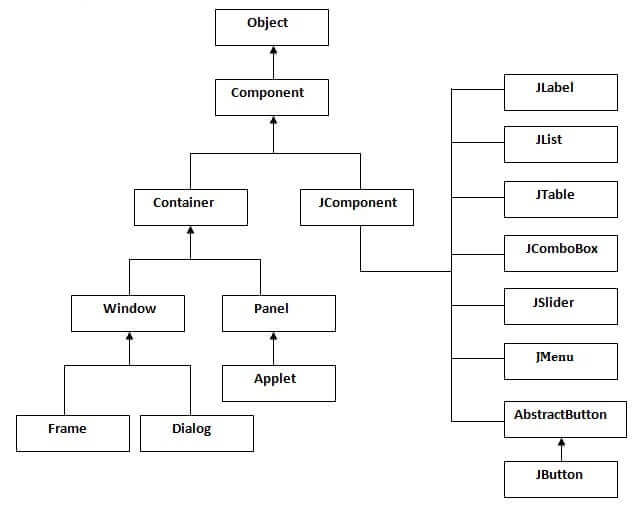
\includegraphics[scale=.7]{Figures/swinghierarchy.jpg}
\end{center}

%------------------------ JOptionPane Class --------------------------
\newpage
\section{Some Important Methods Related to \texttt{JOptionPane} Class}
\begin{table}[!h]
\begin{center}
\begin{tabular}{l|l}
	\hline
	\textbf{Methods Name} & \textbf{Description}\\
	\hline
	showMessageDialog() & Tell the user about something that has happened. \\
	\hline
	showInputDialog() & Prompt for some input.\\
	\hline
	showOptionDialog() & The Grand Unification of the above three.\\
	\hline
	showConfirmDialog() & Asks a confirming question, like yes/no/cancel.\\
	\hline
\end{tabular}
\end{center}
\end{table}

% ----------------- showMessageDialog() Method -----------------------
\subsection{\texttt{showMessageDialog() Method}}
Syntax:\\
\begin{lstlisting}[language=java]
	JOptionPane.showMessageDialog(parameters);
\end{lstlisting}

\begin{itemize}[noitemsep]
	\item \texttt{component, object}
	\item \texttt{component, object, String, int}
	\item \texttt{component, object, String, int, Icon}
\end{itemize}

\textbf{Parameters Descriptions -}
\begin{itemize}[noitemsep]
	\item \texttt{Component –} The first parameter, which determines the Frame in which the dialog is displayed; if null, or if the parentComponent has no Frame, a default Frame is used.
	\item \texttt{Object –} The second parameter can be any objects.
	\item \texttt{String –} The third parameter is a String placed as the title of the message dialog window.
	\item \texttt{int –} The int that follows the String is the MessageType. The different MessageTypes for JOptionPane, are: 
	\begin{itemize}[noitemsep]	
    	\item \texttt{ERROR\_MESSAGE}
    \item \texttt{INFORMATION\_MESSAGE}
    \item \texttt{WARNING\_MESSAGE}
    \item \texttt{QUESTION\_MESSAGE}
    \item \texttt{PLAIN\_MESSAGE}
	\end{itemize}
	\item \texttt{Icon –} The last parameter is an Icon that is displayed inside the dialog and overrides the default MessageType icon.
\end{itemize}

\newpage
\textbf{Example Code:}
\lstset{
  basicstyle=\fontsize{8}{10}\selectfont\ttfamily
}
\begin{lstlisting}[language=java]
package SwingOne;
import javax.swing.ImageIcon;
import javax.swing.JOptionPane;
import java.awt.Image;

class MessageDialog{
	
	public static void main(String[] args) {
		ImageIcon icon = new ImageIcon("D:\\Programming\\Java\\PracticeProject\\Swing\\Icons\\done.png");
		Image image = icon.getImage();
		image = image.getScaledInstance(50, 50, Image.SCALE_SMOOTH);
		icon = new ImageIcon(image);
		JOptionPane.showMessageDialog(null, "Done","Success",JOptionPane.DEFAULT_OPTION, icon);
	}
}
\end{lstlisting}


%-------------------- JOptinPane Icons -----------------------
\subsection{JOptionPane Icons}
\begin{center}
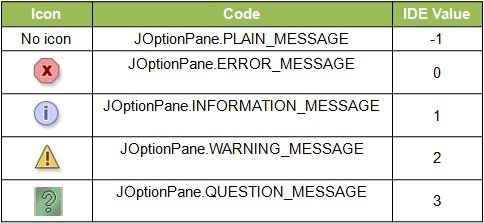
\includegraphics[scale=0.8]{Figures/JOptionPane_Icons.jpg}
\end{center}


%-------------------- showInputDialog() ---------------------
\newpage
\subsection{\texttt{showInputDialog()} Method}
\textbf{Example Code:}
\lstset{
  basicstyle=\fontsize{8}{10}\selectfont\ttfamily
}
\begin{lstlisting}[language=java]
package SwingOne;

import java.awt.Image;
import javax.swing.ImageIcon;
import javax.swing.JOptionPane;

class InputDialog{
	
	public static void main(String[] args) {
		ImageIcon icon = new ImageIcon("D:\\Programming\\Java\\PracticeProject\\Swing\\Icons\\user_Icon.png");
		Image img = icon.getImage();
		img = img.getScaledInstance(50, 50, Image.SCALE_SMOOTH);
		icon = new ImageIcon(img);
		
		String name = JOptionPane.showInputDialog(null,"User Name","User Info",JOptionPane.INFORMATION_MESSAGE);
		int age = 0;
		
		try {
			int birthY = Integer.parseInt(JOptionPane.showInputDialog(null,"Birth Year: ","User Info",JOptionPane.INFORMATION_MESSAGE));
			age = 2023-birthY;
			JOptionPane.showMessageDialog(null,"User Name: "+name+"\nAge: "+age,"User Info",JOptionPane.DEFAULT_OPTION,icon);
		} catch(NumberFormatException e) {
			JOptionPane.showMessageDialog(null,"Invalid Bith Year !!!","Warning",JOptionPane.WARNING_MESSAGE);
		}
		
		
	}
}
\end{lstlisting}



%------------------ showConfirmDialog() Method ----------------------
\newpage
\subsection{\texttt{showConfirmDialog()} Method}

\textbf{Example Code:}
\lstset{
  basicstyle=\fontsize{8}{10}\selectfont\ttfamily
}
\begin{lstlisting}[language=java]
package SwingOne;

import java.awt.Image;
import javax.swing.ImageIcon;
import javax.swing.JOptionPane;

class ConfirmDialog{
	
	public static void main(String[] args) {
		int choice = JOptionPane.showConfirmDialog(null, "Do you want to Execute this Program ?","Confirmation",JOptionPane.YES_NO_OPTION,JOptionPane.QUESTION_MESSAGE);
		
		if(choice == JOptionPane.YES_OPTION) {
			JOptionPane.showMessageDialog(null, "Congratulations !!!","Execute",JOptionPane.INFORMATION_MESSAGE);
		} else {
			JOptionPane.showMessageDialog(null, "Exit program","Exit",JOptionPane.WARNING_MESSAGE);
		}
		
	}
}
\end{lstlisting}


%----------------------------- JFrame ---------------------------
%----------------------------------------------------------------
\newpage
\section{JFrame}

%-------------- Basic JFrame -------------
\subsection{Basic JFrame}
\textbf{Example Code 01:}
\lstset{
  basicstyle=\fontsize{8}{10}\selectfont\ttfamily
}
\begin{lstlisting}[language=java]
package SwingOne;

import javax.swing.JFrame;

class JFrameExample{
	
	public static void main(String[] args) {
		JFrame frame = new JFrame();
		frame.setVisible(true);
		frame.setDefaultCloseOperation(JFrame.EXIT_ON_CLOSE);
		frame.setTitle("Frame Demo");
		frame.setResizable(false);
		
		//----- Set frame size
//		frame.setSize(500,300);
		
		//------ Set frame at center
//		frame.setLocationRelativeTo(null);
		//----- Custom location
//		frame.setLocation(150,70);
		
		//----- Size and Location combine
		//frame.setBounds(left, top, with, height);
		
		frame.setBounds(150,70,500,300);
	}
}
\end{lstlisting}

\textbf{Example Code 02:} Using Constructor.
\lstset{
  basicstyle=\fontsize{8}{10}\selectfont\ttfamily
}
\begin{lstlisting}[language=java]
package SwingOne;

import javax.swing.JFrame;

class JFrameExample extends JFrame{
	
	JFrameExample() {
		setDefaultCloseOperation(JFrame.EXIT_ON_CLOSE);
		setTitle("Frame Demo");
		setBounds(150,100,350,500);
	}
	
	public static void main(String[] args) {
		JFrameExample frame = new JFrameExample();
		frame.setVisible(true);
	}
}
\end{lstlisting}

%-------------- setIconImage() -----------
\newpage
\subsection{Frame Decoration (Icon \& Background Color)}
\textbf{Example Code :}
\lstset{
  basicstyle=\fontsize{8}{10}\selectfont\ttfamily
}
\begin{lstlisting}[language=java]
package SwingOne;

import java.awt.Color;
import java.awt.Container;
import javax.swing.ImageIcon;
import javax.swing.JFrame;

class MakeFrame extends JFrame {
	
	private static final long serialVersionUID = 1L;
	
	private ImageIcon icon = null;
	private Container container = null;

	//------- Constructor
	MakeFrame() {
		setVisible(true);
		setTitle("Frame Demo");
		setDefaultCloseOperation(EXIT_ON_CLOSE);
		setLocationRelativeTo(null);
		setSize(350,500);
		decorateFrame();				// Call decorateFrame() method
	}
	public void decorateFrame() {
		
		//---------- Set Frame Icon ---------------------------
		icon = new ImageIcon(getClass().getResource("done.png"));
		this.setIconImage(icon.getImage());
		
		//----------- Set Frame Background Color ------
		container = this.getContentPane();
//		container.setBackground(Color.ORANGE);
		
		//--------- Set Custom Background Color ------
		Color bgColor = Color.decode("#e6e6fa");
		container.setBackground(bgColor);
	}
}

class JFrameExample{
	
	public static void main(String[] args) {
		MakeFrame frame = new MakeFrame();
		frame.setLocationRelativeTo(null);
	}
}
\end{lstlisting}



%-------------------- JLabel --------------------
\newpage
\section{JLabel}
\subsection{Basic JLabel}
\lstset{
  basicstyle=\fontsize{8}{10}\selectfont\ttfamily
}
\begin{lstlisting}[language=java]
package SwingTwo;

import java.awt.Color;
import java.awt.Container;
import javax.swing.ImageIcon;
import javax.swing.JFrame;
import javax.swing.JLabel;

public class JLabelDemo extends JFrame {

	private static final long serialVersionUID = 1L;
	
	private ImageIcon icon = null;
	private Container container = null;
	private JLabel userLabel = null, passLabel = null;
	
	JLabelDemo() {
		decorateFrame();
	}
	
	public void decorateFrame() {
		
		container = this.getContentPane();
		container.setLayout(null);
		
		icon = new ImageIcon(getClass().getResource("user_Icon.png"));
		this.setIconImage(icon.getImage());
		
		Color bgColor = Color.decode("#e2fbfa");
		container.setBackground(bgColor);
		
		this.setVisible(true);
		this.setTitle("JLabel Demo");
		this.setDefaultCloseOperation(EXIT_ON_CLOSE);
		this.setSize(500,350);
		this.setLocationRelativeTo(null);
		
		userLabel = new JLabel();
		userLabel.setBounds(50,30,100,30);
		userLabel.setText("User Name: ");
		container.add(userLabel);
		
		passLabel = new JLabel("Password: ");
		passLabel.setBounds(50,60,100,30);
		container.add(passLabel);
		
	}

	public static void main(String[] args) {
		JLabelDemo frame = new JLabelDemo();
	}

}
\end{lstlisting}

%-------- Font Style --------
\subsection{JLabel Font Style}

\begin{frame}

\lstset{
  basicstyle=\fontsize{8}{10}\selectfont\ttfamily
}
\begin{lstlisting}[language=java]
class MakeFrame extends JFrame {
	private static final long serialVersionUID = 1L;
	
	private Container container = null;
	private Font robotoFont = null, tnrFont=null;
	private JLabel title = null,userName = null;
	
	MakeFrame() {
		frameDecoration();
	}
	
	public void frameDecoration() {

		container = this.getContentPane();
		container.setLayout(null);
		
		this.setVisible(true);
		this.setTitle("JLable Font Style");
		this.setDefaultCloseOperation(EXIT_ON_CLOSE);
		this.setSize(500,500);
		this.setLocationRelativeTo(null);
		
		//------- Define Font Style
		robotoFont = new Font("Roboto",Font.BOLD,32);
		tnrFont = new Font("Times New Roman",Font.PLAIN,20);
		
		title = new JLabel("User Info");
		title.setBounds(200, 50, 100, 30); 	//	x,y,with,height
		title.setFont(robotoFont);			// Set Font Style
		title.setForeground(Color.RED);		// Change Foreground Color
		title.setOpaque(true);				// Enable to change Background Color
		title.setBackground(Color.BLUE);		// Change Background Color
		container.add(title);				// Add Jlabel to Container
		
		userName = new JLabel("User Name: ");
		userName.setFont(tnrFont);
		userName.setBounds(100,100,100,30);
		container.add(userName);
		
	}
}
\end{lstlisting}

\begin{tikzpicture}[remember picture,overlay]
	\node[anchor=north east] at ([xshift=-1cm,yshift=-5cm]current page.north east) {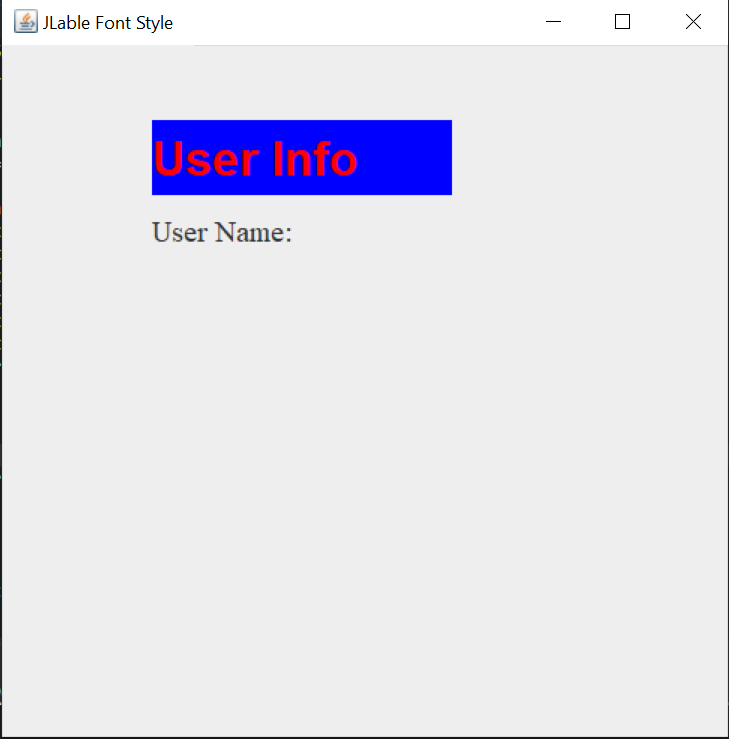
\includegraphics[width=7cm]{Figures/fontStyle.PNG}};
\end{tikzpicture}

\end{frame}


%------ Tip Text -------
\newpage
\subsection{Set Tip Text}

\lstset{
  basicstyle=\fontsize{8}{10}\selectfont\ttfamily
}
\begin{lstlisting}[language=java]
class MakeFrame extends JFrame {
	private static final long serialVersionUID = 1L;
	
	private Container container = null;
	private Font robotoFont = null;
	private JLabel title = null;
	
	MakeFrame() {
		frameDecoration();
	}
	
	public void frameDecoration() {

		container = this.getContentPane();
		container.setLayout(null);
		
		this.setVisible(true);
		this.setTitle("JLable Font Style");
		this.setDefaultCloseOperation(EXIT_ON_CLOSE);
		this.setSize(500,500);
		this.setLocationRelativeTo(null);
		
		//------- Define Font Style
		robotoFont = new Font("Roboto",Font.BOLD,20);
		
		title = new JLabel("User Info");
		title.setToolTipText("Title");		// Tool tip
		title.setBounds(200, 50, 100, 30);
		title.setFont(robotoFont);
		title.setForeground(Color.RED);
		title.setOpaque(true);
		title.setBackground(Color.BLUE);
		container.add(title);
		
	}
}

\end{lstlisting}


%--------- Image Label --------
\newpage
\subsection{Image Label}

\begin{frame}

\lstset{
  basicstyle=\fontsize{8}{10}\selectfont\ttfamily
}
\begin{lstlisting}[language=java]
class MakeFramee extends JFrame {
	private static final long serialVersionUID = 1L;
	
	private Container container = null;
	public JLabel imgLabel = null;
	private ImageIcon icon = null;
	private Image img = null;

	MakeFramee(){
		decorateFrame();
	}
	
	public void decorateFrame() {
		
		container = this.getContentPane();
		container.setLayout(null);
		
		this.setDefaultCloseOperation(EXIT_ON_CLOSE);

		//----- Set Image Label
		icon = new ImageIcon(getClass().getResource("user_Icon.png"));
		img = icon.getImage();
		img = img.getScaledInstance(100, 100, Image.SCALE_SMOOTH); // Resize Image
		icon = new ImageIcon(img);				// Re-assign image to icon
		imgLabel = new JLabel(icon);			// Instantiate image Label
		imgLabel.setBounds(100,100,200,200);
		imgLabel.setOpaque(true);
		imgLabel.setBackground(Color.cyan);
		container.add(imgLabel);				// Add image to container
	}
}

public class ImageLabel {

	public static void main(String[] args) {
		MakeFramee frame = new MakeFramee();
		frame.setVisible(true);
		frame.setTitle("Image Label");
		frame.setBounds(100,50,500,500);
		frame.setLocationRelativeTo(null);
	}

}
\end{lstlisting}

\begin{tikzpicture}[remember picture,overlay]
	\node[anchor=north east] at ([xshift=-1cm,yshift=-3cm]current page.north east) {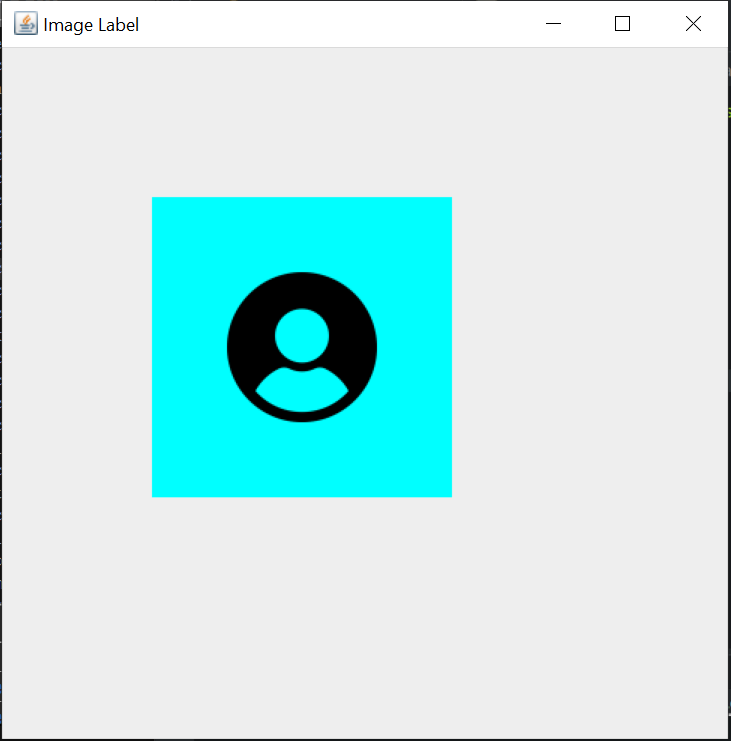
\includegraphics[width=7cm]{Figures/imgLabel.PNG}};
\end{tikzpicture}

\end{frame}


%----------- Text Field ------------
\newpage
\subsection{Text Field}

\begin{frame}

\lstset{
  basicstyle=\fontsize{8}{10}\selectfont\ttfamily
}
\begin{lstlisting}[language=java]
class MKFrame extends JFrame {
	private static final long serialVersionUID = 1L;
	
	private Container container = null;
	private JTextField textField = null;
	
	MKFrame() {
		decorateFrame();		
	}
	
	public void decorateFrame() {
		container = this.getContentPane();
		container.setLayout(null);
		
		this.setTitle("Text Field");
		this.setSize(300,300);
		this.setLocationRelativeTo(null);
		this.setDefaultCloseOperation(EXIT_ON_CLOSE);
		
		font = new Font("Times New Roman",Font.BOLD + Font.ITALIC,18);
		
		textField = new JTextField();
		textField.setFont(font);
		textField.setBounds(50,50,150,50);
		textField.setBackground(Color.cyan);
		textField.setForeground(Color.blue);
		textField.setHorizontalAlignment(JTextField.CENTER); // Writing start form center
		
		container.add(textField);
	}
}

public class TextField {

	public static void main(String[] args) {
		
		MKFrame frame = new MKFrame();
		frame.setVisible(true);

	}

}
\end{lstlisting}

\begin{tikzpicture}[remember picture,overlay]
	\node[anchor=north east] at ([xshift=-1cm,yshift=-2.5cm]current page.north east) {\includegraphics[width=7cm]{Figures/textField.PNG}};
\end{tikzpicture}

\end{frame}


%--------------- Event Listener ---------------------
\newpage
\section{Event Listener}

\subsection{Read text form text field and show in messageDialoug()}

\begin{frame}

\lstset{
  basicstyle=\fontsize{8}{10}\selectfont\ttfamily
}
\begin{lstlisting}[language=java]
class MKFrame extends JFrame {
	private static final long serialVersionUID = 1L;
	
	private Container container = null;
	private JTextField textField = null;
	
	MKFrame() {
		actionListener();
	}
	
	public void actionListener() {
		container = this.getContentPane();
		container.setLayout(null);
		
		this.setTitle("Event Listener");
		this.setSize(300,300);
		this.setLocationRelativeTo(null);
		this.setDefaultCloseOperation(EXIT_ON_CLOSE);
		
		textField = new JTextField();
		textField.setBounds(50,50,150,50);
		
		container.add(textField);
		
		//----------------- Event Listener
		textField.addActionListener(new ActionListener() {
			public void actionPerformed(ActionEvent e) {
				String msg = textField.getText();	// Get message from textField
				textField.setText("Done");			// Replace text with "Done" msg
				if(!(msg.isEmpty())) {
					JOptionPane.showMessageDialog(null, msg);
				} else {
					JOptionPane.showMessageDialog(null, "Empty Message !");
				}
			}
		});
	}
}

public class TextField {
	public static void main(String[] args) {
		
		MKFrame frame = new MKFrame();
		frame.setVisible(true);
	}
}
\end{lstlisting}

\begin{tikzpicture}[remember picture,overlay]
	\node[anchor=north east] at ([xshift=-1cm,yshift=-4.5cm]current page.north east) {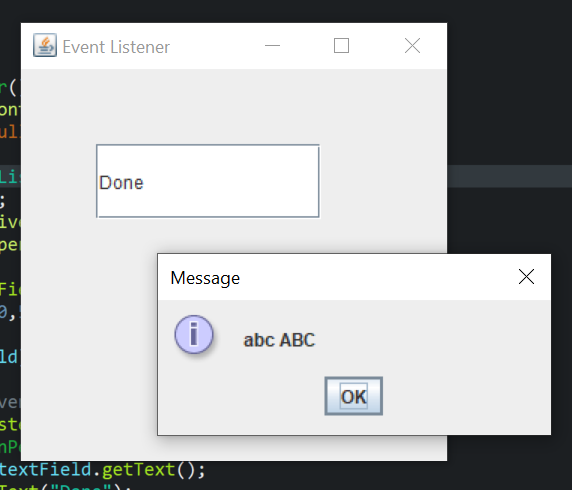
\includegraphics[width=7cm]{Figures/eventListener.PNG}};
\end{tikzpicture}

\end{frame}

%-------------------------------------
\subsection{Perform EventListener for JTextField and Show Message Using showMessageDialog}

\begin{frame}

\lstset{
  basicstyle=\fontsize{8}{10}\selectfont\ttfamily
}
\begin{lstlisting}[language=java]
class MakeFrame extends JFrame {
	private static final long serialVersionUID = 1L;
	
	private Container container = null;
	private JLabel heading = null;
	private JTextField nameField = null, IdField = null;
	private Font font = null;
	
	MakeFrame(int width, int height) {
		this.setTitle("Event Listener");
		this.setSize(width,height);
		this.setLocationRelativeTo(null);
		this.setDefaultCloseOperation(EXIT_ON_CLOSE);
		frameActions();
	}
	
	public void frameActions() {
		container = this.getContentPane();
		container.setLayout(null);
		
		font = new Font("Times New Roman",Font.BOLD,20);
		
		// Crate and add JLabel to the container
		heading = new JLabel("Name and ID");
		heading.setFont(font);
		heading.setBounds(160,50,150,30);
		container.add(heading);
		
		font = new Font("Times New Roman",Font.PLAIN,16);
		
		// Configure and add JTextField to the Container
		nameField = new JTextField();
		nameField.setBounds(100,100,300,30);
		nameField.setFont(font);
		container.add(nameField);
		
		IdField = new JTextField();
		IdField.setBounds(100,150,300,30);
		IdField.setFont(font);
		container.add(IdField);
		
		// Instantiate EventHandler Class and pass the JTextFields as parameter
		EventHandler eventHandler = new EventHandler(nameField, IdField);
		
		nameField.addActionListener(eventHandler);
		IdField.addActionListener(eventHandler);
	}
}

// Implements the ActionListner interface
class EventHandler implements ActionListener {
	
	private JTextField nameField = null, idField = null;
	
	EventHandler(JTextField name, JTextField Id) {
		nameField = name;
		idField = Id;
	}
	
	public void actionPerformed(ActionEvent e) {
		String str = null;
		if(e.getSource() == nameField) {
			str = nameField.getText();
			if(str.isEmpty()) {
				JOptionPane.showMessageDialog(null, "Empty Name Field","Name Field",JOptionPane.WARNING_MESSAGE);
			} else {
				JOptionPane.showMessageDialog(null, str,"Name Field",JOptionPane.PLAIN_MESSAGE);
			}
		} else {
			str = idField.getText();
			if(str.isEmpty()) {
				JOptionPane.showMessageDialog(null, "Empty Id Field","Id Field",JOptionPane.WARNING_MESSAGE);
			} else {
				JOptionPane.showMessageDialog(null, str, "Id Field", JOptionPane.PLAIN_MESSAGE);
			}
		}
	}
}

public class EventListener1 {

	public static void main(String[] args) {
		MakeFrame frame = new MakeFrame(500,500);
		frame.setVisible(true);
	}

}
\end{lstlisting}

\begin{tikzpicture}[remember picture,overlay]
	\node[anchor=north east] at ([xshift=-1.2cm,yshift=-15cm]current page.north east) {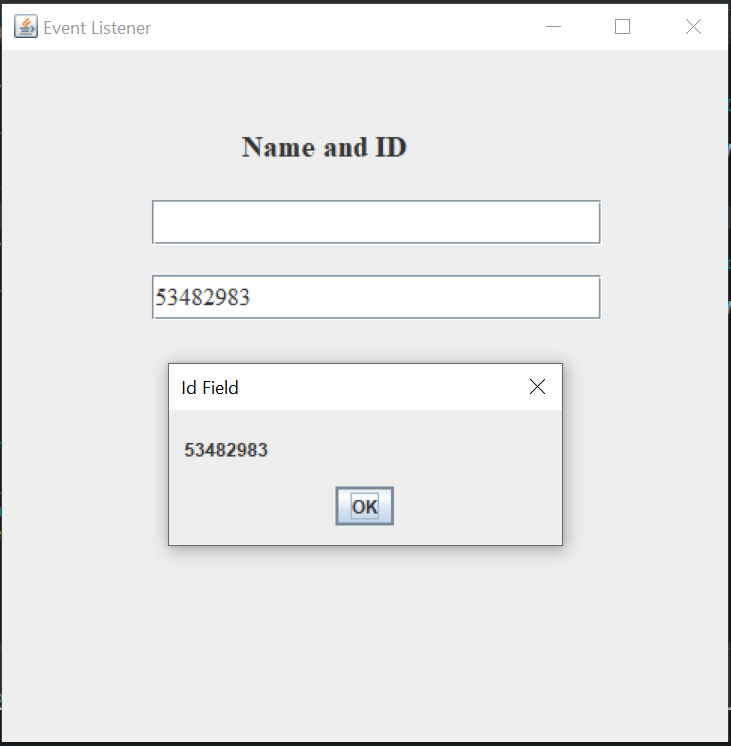
\includegraphics[width=7cm]{Figures/eventListener2.PNG}};
\end{tikzpicture}

\end{frame}


%--------------- Pass Field -------------
\newpage
\subsection{Password Field}

\begin{frame}

\lstset{
  basicstyle=\fontsize{8}{10}\selectfont\ttfamily
}
\begin{lstlisting}[language=java]
class CreatFrame extends JFrame{
	private static final long serialVersionUID = 1L;
	
	private Container container = null;
	private JPasswordField passField = null;
	
	CreatFrame() {
		this.setTitle("Password Field");
		this.setSize(500,500);
		this.setDefaultCloseOperation(EXIT_ON_CLOSE);
		this.setLocationRelativeTo(null);
		frameActions();
	}
	
	public void frameActions() {
		container = this.getContentPane();
		container.setLayout(null);
		
		JLabel label = new JLabel("Enter Password");
		label.setBounds(100,100,200,30);
		container.add(label);
		
		passField = new JPasswordField();
		passField.setBounds(100,130,200,30);
		passField.setEchoChar('#');
		container.add(passField);
		
	}
}

public class PasswordField {
	public static void main(String[] args) {
		CreatFrame frame = new CreatFrame();
		frame.setVisible(true);
	}
}
\end{lstlisting}

\begin{tikzpicture}[remember picture,overlay]
	\node[anchor=north east] at ([xshift=-1cm,yshift=-4.5cm]current page.north east) {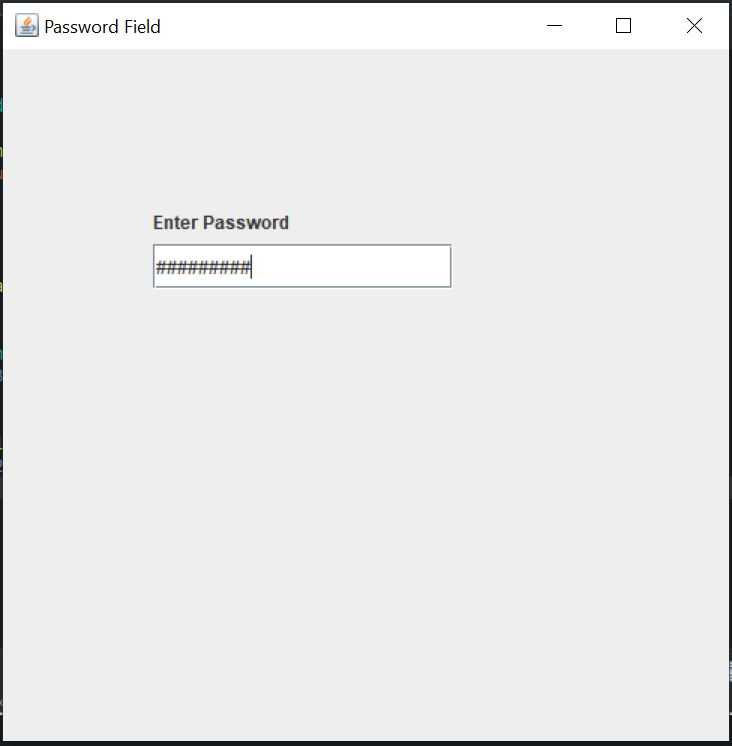
\includegraphics[width=7cm]{Figures/passField.PNG}};
\end{tikzpicture}

\end{frame}


%--------------- Button Field -------------
\newpage
\subsection{Button Field}

\begin{frame}

\lstset{
  basicstyle=\fontsize{8}{10}\selectfont\ttfamily
}
\begin{lstlisting}[language=java]
class BuildFrame extends JFrame {
	private static final long serialVersionUID = 1L;
	
	private Container container = null;
	private JButton button = null;
	
	BuildFrame () {
		this.setTitle("Button Field");
		this.setSize(500,500);
		this.setLocationRelativeTo(null);
		frameActions();
	}
	
	public void frameActions() {
		container = this.getContentPane();
		container.setLayout(null);
		
		button = new JButton("Submit");
		button.setSize(100,50);
		button.setLocation(200,200);
		container.add(button);
	}
}

public class ButtonField {

	public static void main(String[] args) {
		
		BuildFrame frame = new BuildFrame();
		frame.setVisible(true);
	}
}
\end{lstlisting}

\begin{tikzpicture}[remember picture,overlay]
	\node[anchor=north east] at ([xshift=-1cm,yshift=-5cm]current page.north east) {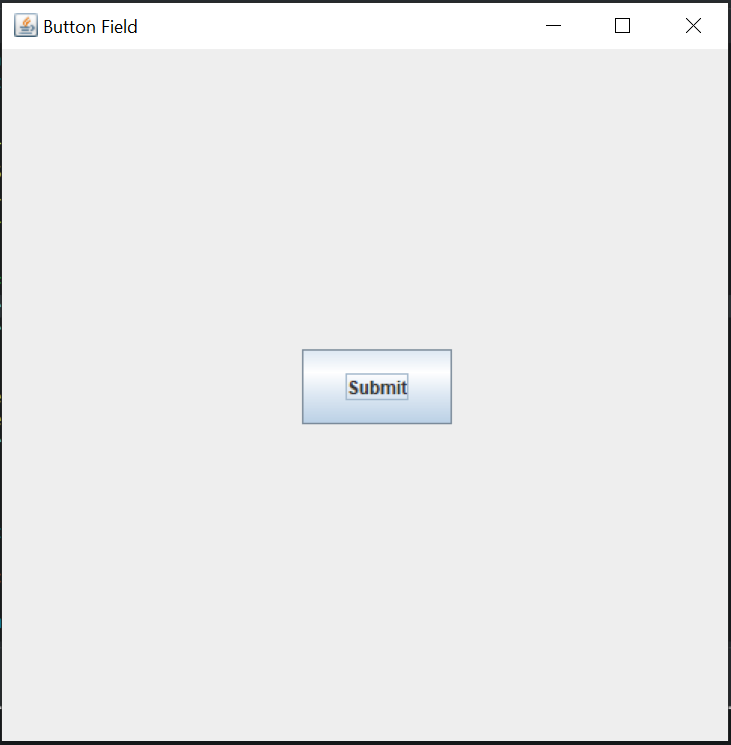
\includegraphics[width=7cm]{Figures/button.PNG}};
\end{tikzpicture}

\end{frame}



%-------- Drawing Shapes -------------
\newpage
\section{Drawing Shapes}

\begin{frame}

\lstset{
  basicstyle=\fontsize{8}{10}\selectfont\ttfamily
}
\begin{lstlisting}[language=java]
DrawingPanel() {
		
		this.setTitle("Drawing Shapes");
		this.setSize(500,500);
		this.setLocationRelativeTo(null);
		this.setDefaultCloseOperation(EXIT_ON_CLOSE);
		
		JPanel drawintPanel = new JPanel() {
			public void paintComponent(Graphics g) {
				Graphics2D g2 = (Graphics2D) g;
				
				//Rectangle2D.Double(x,y,width,height);
				Shape rect = new Rectangle2D.Double(100,100,300,250);
				g2.setColor(Color.GREEN);
				g2.fill(rect);
				
				// Ellipse2D.Double(x,y,width,height);
				Shape circle = new Ellipse2D.Double(110,50,100,100);
				g2.setColor(Color.blue);
				g2.fill(circle);
				
				// Draw line form (x1,y2) to (x2,y2)
				Shape line = new Line2D.Double(130,25,130,300);
				g2.setStroke(new BasicStroke(10));
				g2.setColor(Color.red);
				g2.draw(line);	
			}
		};
		
		this.getContentPane().add(drawintPanel);
		this.setVisible(true);
	}
}

public class DrawingApp {
	public static void main(String[] args) {
		DrawingPanel frame = new DrawingPanel();
	}
}
\end{lstlisting}

\begin{tikzpicture}[remember picture,overlay]
	\node[anchor=north east] at ([xshift=-1cm,yshift=-15cm]current page.north east) {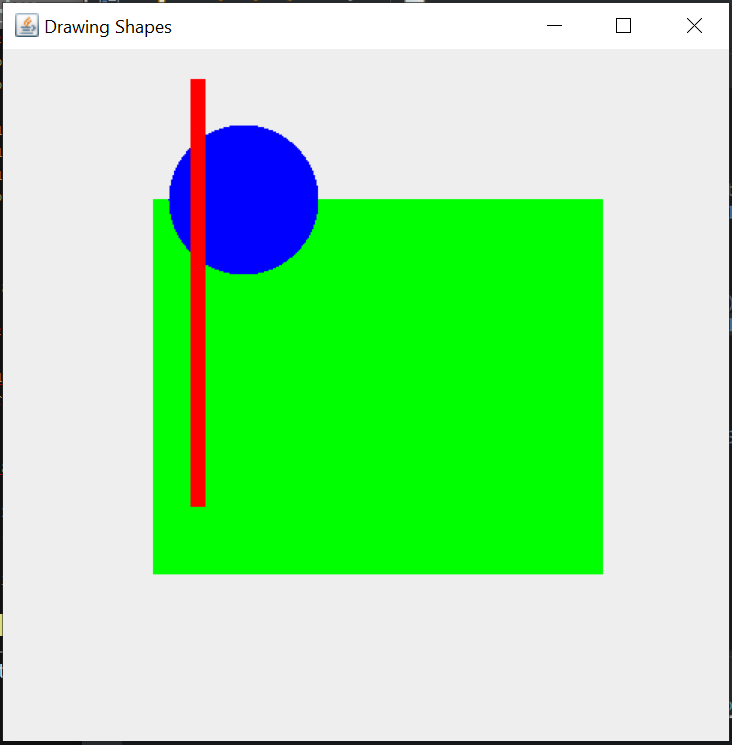
\includegraphics[width=7cm]{Figures/drawShape.PNG}};
\end{tikzpicture}

\end{frame}


%-------- Curors -------------
\newpage
\section{Set Cursor}

\begin{frame}

\AddToShipoutPictureFG*{ % Add figure to foreground of current page
  \put(\LenToUnit{13cm},\LenToUnit{17cm}){% Adjust the coordinates as needed
    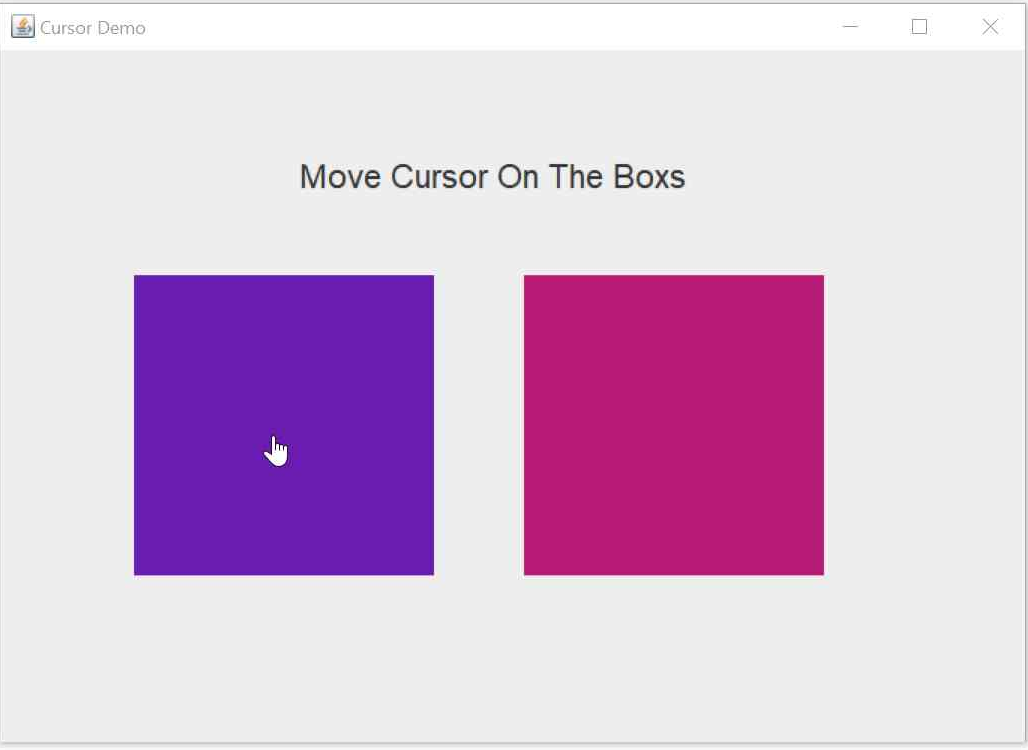
\includegraphics[width=7cm]{Figures/cursor1.png}
  }
}

\AddToShipoutPictureFG*{ % Add figure to foreground of current page
  \put(\LenToUnit{13cm},\LenToUnit{5cm}){% Adjust the coordinates as needed
    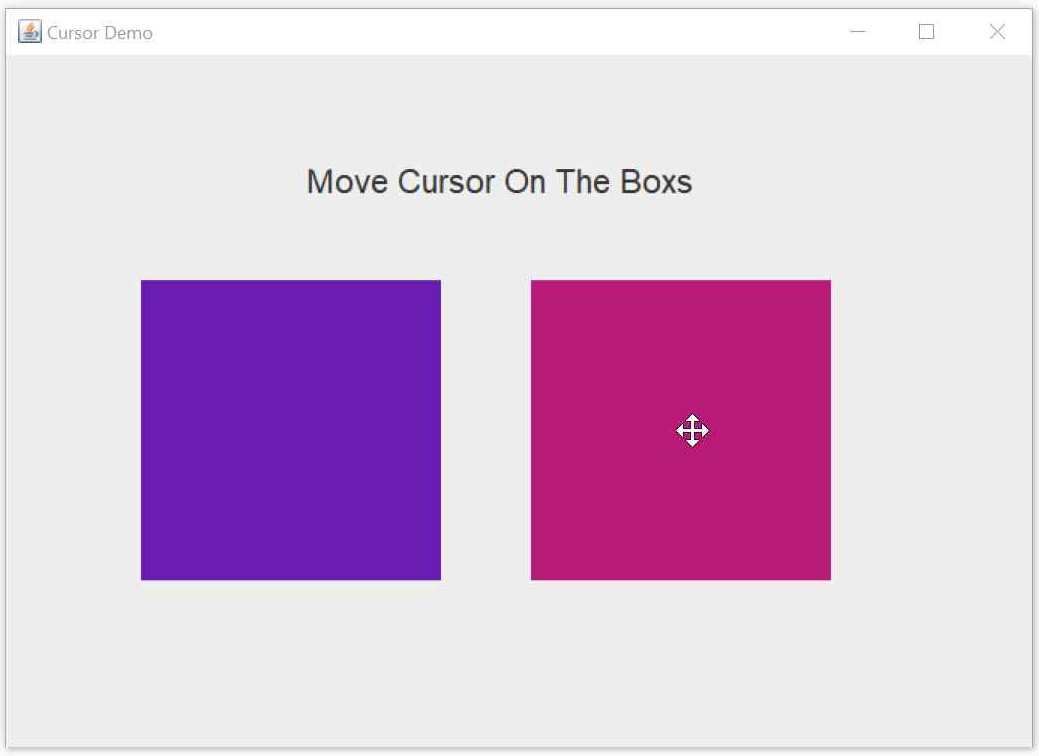
\includegraphics[width=7cm]{Figures/cursor2.png}
  }
}

\lstset{
  basicstyle=\fontsize{8}{10}\selectfont\ttfamily
}
\begin{lstlisting}[language=java]

package SwingTwo;

import java.awt.*;

import javax.swing.*;

public class CursorDemo extends JFrame {
	private static final long serialVersionUID = 1L;
	
	private Container container;
	private JLabel heading, label1, label2;
	private Font font;
	private Cursor cursor1, cursor2;
	
	CursorDemo() {
		this.setTitle("Cursor Demo");
		this.setSize(700,500);
		this.setLocationRelativeTo(null);
		this.setDefaultCloseOperation(JFrame.EXIT_ON_CLOSE);
		initComponents();
	}
	
	public void initComponents() {
		
		font = new Font("Arial",Font.PLAIN,22);
		cursor1 = new Cursor(Cursor.HAND_CURSOR);
		cursor2 = new Cursor(Cursor.MOVE_CURSOR);
		
		container = this.getContentPane();
		container.setLayout(null);
		
		//----- Heading Label
		heading = new JLabel("Move Cursor On The Boxs");
		heading.setFont(font);
		heading.setBounds(200,70,300,30);
		container.add(heading);
		
		//--- Label 1
		label1 = new JLabel();
		label1.setFont(font);
		label1.setBounds(90,150,200,200);
		label1.setOpaque(true);
		label1.setBackground(Color.decode("#6a1cb0"));
		label1.setCursor(cursor1); // Add cursor
		container.add(label1);
		
		
		
		
		//--- Label 2
		label2 = new JLabel();
		label2.setFont(font);
		label2.setBounds(350,150,200,200);
		label2.setOpaque(true);
		label2.setBackground(Color.decode("#b71b77"));
		label2.setCursor(cursor2);	// Add cursor
		container.add(label2);
		
	}

	public static void main(String[] args) {
		
		CursorDemo frame = new CursorDemo();
		frame.setVisible(true);
	}

}
\end{lstlisting}

\end{frame}



	\chapter{Latex Ticks}

\section{Figure Overlap On The Plain Text}

\begin{frame}

\lstset{
  basicstyle=\fontsize{8}{10}\selectfont\ttfamily
}
\begin{lstlisting}[language=java]
class MakeFramee extends JFrame {
	
	private Container container = null;
	public JLabel imgLabel = null;
	private ImageIcon icon = null;
	private Image img = null;

	MakeFramee(){
		decorateFrame();
	}
	
	public void decorateFrame() {
		
		container = this.getContentPane();
		container.setLayout(null);
		
		this.setDefaultCloseOperation(EXIT_ON_CLOSE);

		//----- Set Image Label
		icon = new ImageIcon(getClass().getResource("user_Icon.png"));
		img = icon.getImage();
		img = img.getScaledInstance(100, 100, Image.SCALE_SMOOTH); // Resize Image
		icon = new ImageIcon(img);				// Re-assign image to icon
		imgLabel = new JLabel(icon);			// Instantiate image Label
		imgLabel.setBounds(100,100,200,200);
		imgLabel.setOpaque(true);
		imgLabel.setBackground(Color.cyan);
		container.add(imgLabel);				// Add image to container
	}
}

\end{lstlisting}

\begin{tikzpicture}[remember picture,overlay]
	\node[anchor=north east] at ([xshift=-1cm,yshift=-7cm]current page.north east) {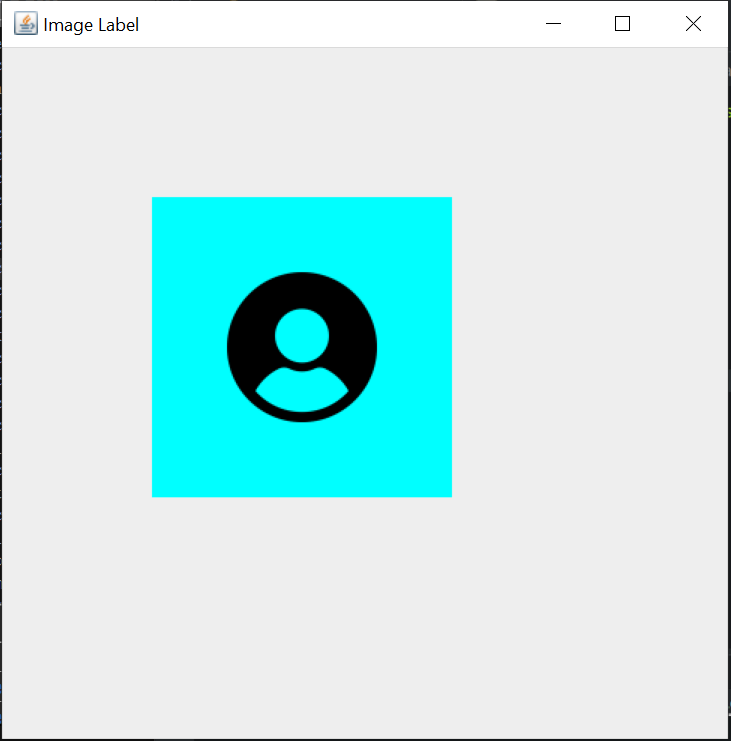
\includegraphics[width=7cm]{Figures/imgLabel.PNG}};
\end{tikzpicture}

\end{frame}



%--------------- Efficient Control Over the figure ----------------
\newpage
\section{More Control over the Figure }
\begin{frame}

\AddToShipoutPictureFG*{ % Add figure to foreground of current page
  \put(\LenToUnit{13cm},\LenToUnit{7cm}){% Adjust the coordinates as needed
    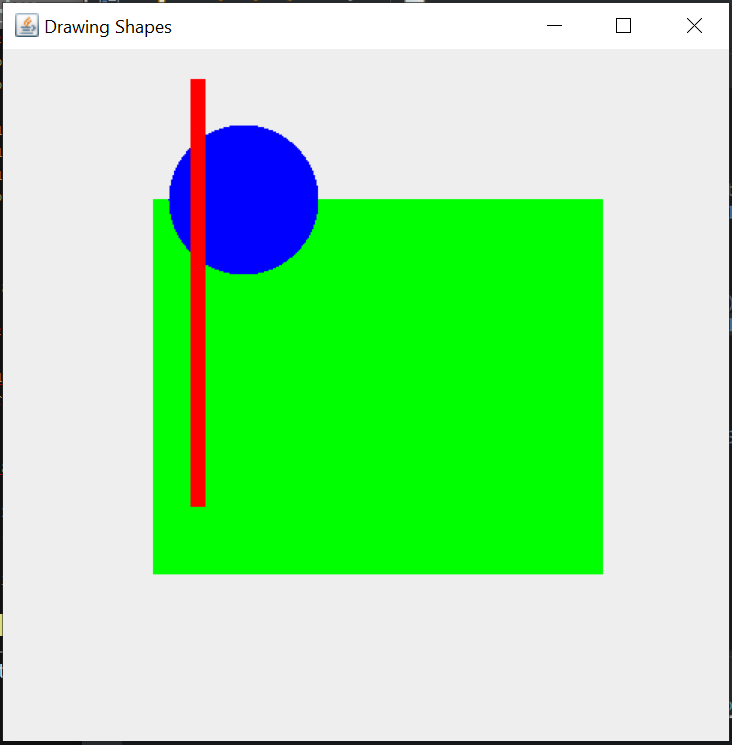
\includegraphics[width=7cm]{Figures/drawShape.PNG}
  }
}

\lstset{
  basicstyle=\fontsize{8}{10}\selectfont\ttfamily,
  numberstyle=\tiny\color{codegray}
}
\begin{lstlisting}[language=java]
DrawingPanel() {
		
		this.setTitle("Drawing Shapes");
		this.setSize(500,500);
		this.setLocationRelativeTo(null);
		this.setDefaultCloseOperation(EXIT_ON_CLOSE);
		
		JPanel drawintPanel = new JPanel() {
			public void paintComponent(Graphics g) {
				Graphics2D g2 = (Graphics2D) g;
				
				//Rectangle2D.Double(x,y,width,height);
				Shape rect = new Rectangle2D.Double(100,100,300,250);
				g2.setColor(Color.GREEN);
				g2.fill(rect);
				
				// Ellipse2D.Double(x,y,width,height);
				Shape circle = new Ellipse2D.Double(110,50,100,100);
				g2.setColor(Color.blue);
				g2.fill(circle);
				
				// Draw line form (x1,y2) to (x2,y2)
				Shape line = new Line2D.Double(130,25,130,300);
				g2.setStroke(new BasicStroke(10));
				g2.setColor(Color.red);
				g2.draw(line);	
			}
		};
		
		this.getContentPane().add(drawintPanel);
		this.setVisible(true);
	}
}

public class DrawingApp {
	public static void main(String[] args) {
		DrawingPanel frame = new DrawingPanel();
	}
}

\end{lstlisting}


\end{frame}

	
	
\end{document}